\documentclass[border=3pt]{standalone}
% Preâmbulo compartilhado pelos diagramas TikZ da aula 11 (Localização por Grade e Monte Carlo)
\usepackage[T1]{fontenc}
\usepackage[utf8]{inputenc}
\usepackage{lmodern}
\usepackage{amsmath}
\usepackage{xcolor}
\usepackage{tikz}
\usetikzlibrary{arrows.meta,angles,quotes,decorations.pathmorphing,calc,
                positioning,shapes.geometric,shapes.misc,backgrounds,fit,
                math}

% Paleta (mesma dos SVGs originais)
\definecolor{dblue}{HTML}{2A5B8C}
\definecolor{dorange}{HTML}{B3541E}
\definecolor{dgreen}{HTML}{4A7C59}
\definecolor{dred}{HTML}{9C4B4B}
\definecolor{dcream}{HTML}{F4F1EA}
\definecolor{dshade}{HTML}{DDD7C9}

% Função gaussiana (não normalizada por padrão de escala visual)
\pgfmathdeclarefunction{gauss}{3}{%
  \pgfmathparse{1/(#3*sqrt(2*pi))*exp(-((#1-#2)^2)/(2*#3^2))}%
}

% Estilos comuns (prefixo d... para não colidir com chaves internas do pgf)
\tikzset{
  >={Stealth[length=2mm]},
  dguide/.style={gray!55, dashed, line width=0.4pt},
  daxis/.style={gray!60, line width=0.7pt, ->},
  dbody/.style={fill=black!3, draw=black!80, line width=1pt},
  dacc/.style={draw=dblue, line width=1pt},
  dlbl/.style={black!55, font=\small},
  dsub/.style={black!45, font=\footnotesize},
  dstate/.style={circle, draw=black!80, fill=dcream, line width=1pt,
                 minimum size=17mm, font=\large, inner sep=1pt},
  dobs/.style={circle, draw=black!80, fill=dshade, line width=1pt,
               minimum size=14mm, font=\large, inner sep=1pt},
  dbox/.style={rounded corners=2pt, draw=black!80, fill=dcream, line width=1pt,
               align=center, inner sep=6pt},
  dop/.style={circle, draw=black!80, fill=white, line width=1pt,
              minimum size=6mm, inner sep=0pt, font=\small},
  dtrans/.style={->, dblue, line width=1pt},
  dmeas/.style={->, dorange, line width=1pt},
  dcurve/.style={line width=1pt, dblue},
  dcurveb/.style={line width=1.4pt, dorange},
}

\begin{document}
\hyphenpenalty=10000 \exhyphenpenalty=10000 \tolerance=9999 \emergencystretch=3em
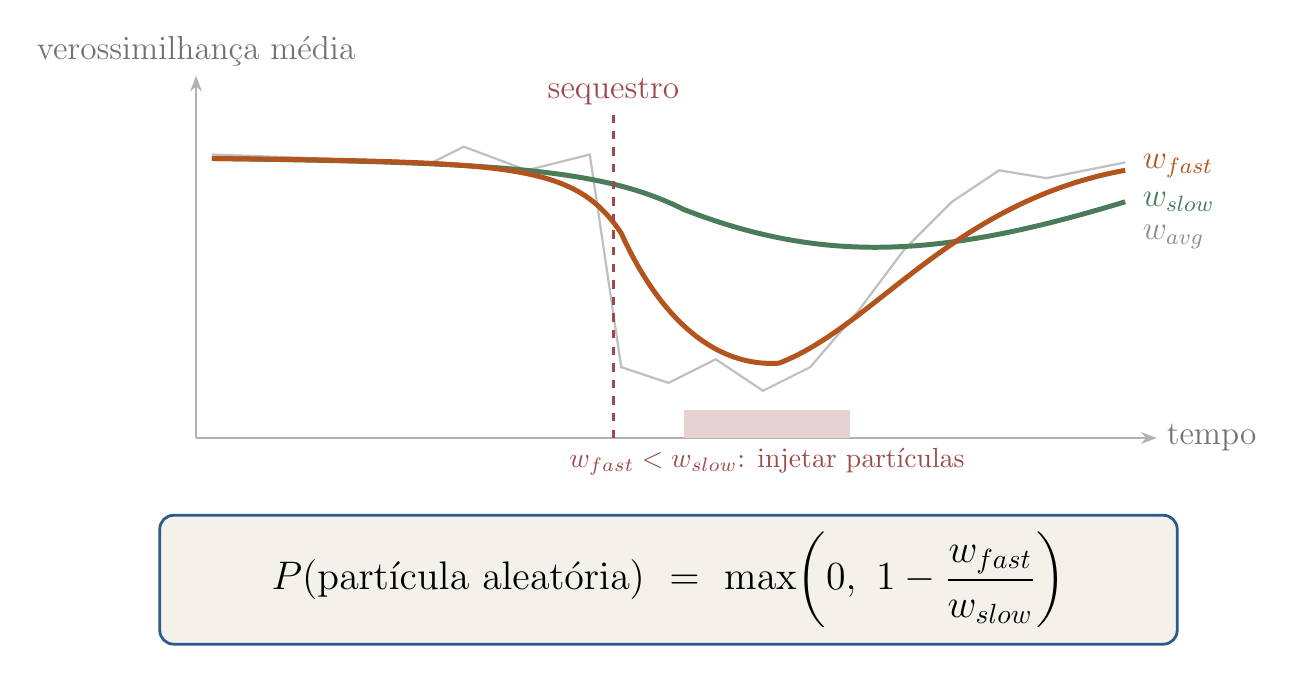
\begin{tikzpicture}[x=1cm,y=1cm]
  \draw[daxis] (0,0) -- (12.2,0) node[right, dlbl, font=\large] {tempo};
  \draw[daxis] (0,0) -- (0,4.6) node[above, dlbl, font=\large] {verossimilhança média};
  \draw[black!25, line width=0.8pt] (0.2,3.6) -- (3,3.5) -- (3.4,3.7) -- (4.2,3.4) -- (5.0,3.6) -- (5.4,0.9) -- (6.0,0.7) -- (6.6,1.0) -- (7.2,0.6) -- (7.8,0.9) -- (8.4,1.6) -- (9.0,2.4) -- (9.6,3.0) -- (10.2,3.4) -- (10.8,3.3) -- (11.8,3.5);
  \draw[dgreen, line width=1.8pt] (0.2,3.55) .. controls (4,3.5) and (5.2,3.4) .. (6.2,2.9) .. controls (8,2.2) and (9.5,2.3) .. (11.8,3.0);
  \draw[dorange, line width=1.8pt] (0.2,3.55) .. controls (4,3.5) and (4.8,3.5) .. (5.4,2.6) .. controls (5.9,1.5) and (6.6,0.9) .. (7.4,0.95) .. controls (8.6,1.4) and (9.6,3.0) .. (11.8,3.4);
  \draw[dred, dashed, line width=1.2pt] (5.3,0) -- (5.3,4.1); \node[dred, font=\large, anchor=south] at (5.3,4.1) {sequestro};
  \fill[dred!25] (6.2,0) rectangle (8.3,0.35);
  \node[dred, font=\normalsize, anchor=north] at (7.25,0) {$w_{fast} < w_{slow}$: injetar partículas};
  \node[dorange, font=\large, anchor=west] at (11.9,3.45) {$w_{fast}$};
  \node[dgreen, font=\large, anchor=west] at (11.9,3.0) {$w_{slow}$};
  \node[black!45, font=\large, anchor=west] at (11.9,2.55) {$w_{avg}$};
  \node[dbox, rounded corners=5pt, text width=12.5cm, font=\Large, draw=dblue] at (6,-1.8) {$P(\text{partícula aleatória}) = \max\!\left(0,\ 1 - \dfrac{w_{fast}}{w_{slow}}\right)$};
\end{tikzpicture}
\end{document}
